\documentclass[11pt]{charter}

% El títulos de la memoria, se usa en la carátula y se puede usar el cualquier lugar del documento con el comando \ttitle
\titulo{Medición y aceptación de parámetros en transformadores de corriente alterna} 

% Nombre del posgrado, se usa en la carátula y se puede usar el cualquier lugar del documento con el comando \degreename
\posgrado{Carrera de Especialización en Sistemas Embebidos} 
%\posgrado{Carrera de Especialización en Internet de las Cosas} 
%\posgrado{Carrera de Especialización en Intelegencia Artificial}
%\posgrado{Maestría en Sistemas Embebidos} 
%\posgrado{Maestría en Internet de las cosas}

% Tu nombre, se puede usar el cualquier lugar del documento con el comando \authorname
\autor{Cristian Trinidad} 

% El nombre del director y co-director, se puede usar el cualquier lugar del documento con el comando \supname y \cosupname y \pertesupname y \pertecosupname
\director{Esp. Lic. Leopoldo A. Zimperz}
\pertenenciaDirector{Iris Tecnologia S.R.L.} 
% FIXME:NO IMPLEMENTADO EL CODIRECTOR ni su pertenencia
\codirector{} % si queda vacio no se deberíá incluir 
\pertenenciaCoDirector{}

% Nombre del cliente, quien va a aprobar los resultados del proyecto, se puede usar con el comando \clientename y \empclientename
\cliente{Esp. Lic. Leopoldo A. Zimperz}
\empresaCliente{Iris Tecnologia S.R.L.}

% Nombre y pertenencia de los jurados, se pueden usar el cualquier lugar del documento con el comando \jurunoname, \jurdosname y \jurtresname y \perteunoname, \pertedosname y \pertetresname.
\juradoUno{Nombre y Apellido (1)}
\pertenenciaJurUno{pertenencia (1)} 
\juradoDos{Nombre y Apellido (2)}
\pertenenciaJurDos{pertenencia (2)}
\juradoTres{Nombre y Apellido (3)}
\pertenenciaJurTres{pertenencia (3)}
 
\fechaINICIO{22 de junio de 2020}		%Fecha de inicio de la cursada de GdP \fechaInicioName
\fechaFINALPlanificacion{22 de Agosto de 2020} 	%Fecha de final de cursada de GdP
\fechaFINALTrabajo{22 de diciembre de 2020}		%Fecha de defensa pública del trabajo final


\begin{document}

\maketitle
\thispagestyle{empty}
\pagebreak


\thispagestyle{empty}
{\setlength{\parskip}{0pt}
\tableofcontents{}
}
\pagebreak


\section{Registros de cambios}
\label{sec:registro}


\begin{table}[ht]
\label{tab:registro}
\centering

\begin{tabularx}{\linewidth}{@{}|c|X|c|@{}}
\hline
\rowcolor[HTML]{C0C0C0} 
Revisión & \multicolumn{1}{c|}{\cellcolor[HTML]{C0C0C0}Detalles de los cambios realizados} & Fecha      \\ \hline
1.0      & Creación del documento                                                          & 22/06/2020 \\ \hline
1.1      & Ejemplo de un texto muy largo que debiera ocupar más de una línea para que tengan de ejemplo                                                                                																						   & dd/mm/aaaa \\ \hline
1.2      & Otro ejemplo \newline
		   Con texto partido \newline
		   En varias líneas \newline
		   A propósito                                                                     & dd/mm/aaaa \\ \hline
\end{tabularx}
\end{table}

\pagebreak



\section{Acta de Constitución del Proyecto}
\label{sec:acta}

\begin{flushright}
Buenos Aires, \fechaInicioName
\end{flushright}

\vspace{2cm}

Por medio de la presente se acuerda con el Ing. \authorname\hspace{1px} que su Trabajo Final de la \degreename\hspace{1px} se titulará ``\ttitle'', consistirá esencialmente en el prototipo preliminar de un dispositivo capaz de medir y registrar parámetros de transformadores de corriente alterna empleados en la fabricación de dispositivos electromédicos, y tendrá un presupuesto preliminar estimado de 600 hs de trabajo y \textcolor{red}{\$XXX}, con fecha de inicio \fechaInicioName\hspace{1px} y fecha de presentación pública \fechaFinalName.

Se adjunta a esta acta la planificación inicial.

\vfill

% Esta parte se construye sola con la información que hayan cargado en el preámbulo del documento y no debe modificarla
\begin{table}[ht]
\centering
\begin{tabular}{ccc}
\begin{tabular}[c]{@{}c@{}}Ariel Lutenberg \\ Director posgrado FIUBA\end{tabular} &  & \begin{tabular}[c]{@{}c@{}}\clientename \\ \empclientename \end{tabular} \vspace{2.5cm} \\ 
\multicolumn{3}{c}{\begin{tabular}[c]{@{}c@{}} \supname \\ Director del Trabajo Final\end{tabular}} \vspace{2.5cm} \\
\begin{tabular}[c]{@{}c@{}}\jurunoname \\ Jurado del Trabajo Final\end{tabular}     &  & \begin{tabular}[c]{@{}c@{}}\jurdosname\\ Jurado del Trabajo Final\end{tabular}  \vspace{2.5cm}  \\
\multicolumn{3}{c}{\begin{tabular}[c]{@{}c@{}} \jurtresname\\ Jurado del Trabajo Final\end{tabular}} \vspace{.5cm}                                                                     
\end{tabular}
\end{table}




\section{Descripción técnica-conceptual del Proyecto a realizar}
\label{sec:descripcion}


La empresa Iris tecnología S.R.L. fabrica equipos electromédicos cumpliendo con los requisitos de Buenas Prácticas de Fabricación exigidos por la Administración Nacional de Medicamentos, Alimentos y Tecnología Médica (A.N.M.A.T.). Adicionalmente, incorporó recientemente un sistema de gestión de calidad para fabricación de dispositivos médicos, basado en la norma ISO13485:2016. En la actualidad se está trabajando en la incorporación de tecnologías para agilizar tareas y controles que deben realizarse acorde a dicho sistema de calidad. 

Entre las tareas y controles antes mencionados se encuentra el ensayo y calificación de  transformadores para su posterior utilización en las líneas de producción. El objetivo de este proyecto es proveer un dispositivo capaz de automatizar este procedimiento que, actualmente, se realiza en forma manual. Esta labor además de insumir una gran cantidad de tiempo y ser muy repetitiva, presenta un gran riesgo de error humano, y puede además, comprometer la seguridad del operario y la fiabilidad de los datos obtenidos.

La idea es desarrollar un prototipo capaz de medir y registrar los parámetros de transformadores de tensión alterna empleados en la fabricación de dispositivos electromédicos, a fin ser aceptados o rechazados para su posterior uso. Los parámetros a medir incluyen las tensiones y corrientes de los bobinados primario y secundario.

En la Figura \ref{fig:diagBloques} se presenta el diagrama en bloques del sistema. En la figura se destaca el dispositivo a diseñar dentro del recuadro, adicionalmente se incluyen el transformador a ensayar y las fuentes de corriente alternas externas. Dentro del dispositivo a diseñar se observan los siguientes bloques principales:

\begin{itemize}
\item Módulo ESP32 con WiFi integrado.
\item Bloques de acondicionamiento de señal y actuación para el bobinado primario y secundario.
\item Interfaz de usuario: pulsadores, display y \textit{buzzer}.
\item Interfaz para impresora RS232.
\item \textit{Switch} de seguridad para indicar que la tapa de seguridad ha sido removida.
\item Fuente de alimentación.
\end{itemize}

El dispositivo propuesto deberá indicar al operador si el transformador es aceptado o rechazado en base a umbrales previamente configurados por medio de una comunicación WiFi. Además de mostrar el resultado del ensayo localmente, este y las mediciones realizadas deberán ser enviados a un servidor web a través de la comunicación WiFi y adicionalmente se debe imprimir una etiqueta que permita la trazabilidad del componente.

A continuación se presenta un resumen de las tareas propuestas para el dispositivo a desarrollar:
\begin{itemize}
\item Mediciones de tensión y corriente a los transformadores bajo ensayo.
\item Configuración de umbrales de aceptación para los parámetros medidos.
\item Emitir confirmación de aceptación o rechazo del transformador.
\item Visualización en display LCD de umbrales seteados y mediciones.
\item Envío de las mediciones a servidor web, vía red WiFi.
\item Impresión de etiquetas con número de partida y valores medidos. 
\end{itemize}

\begin{figure}[htpb]
\centering 
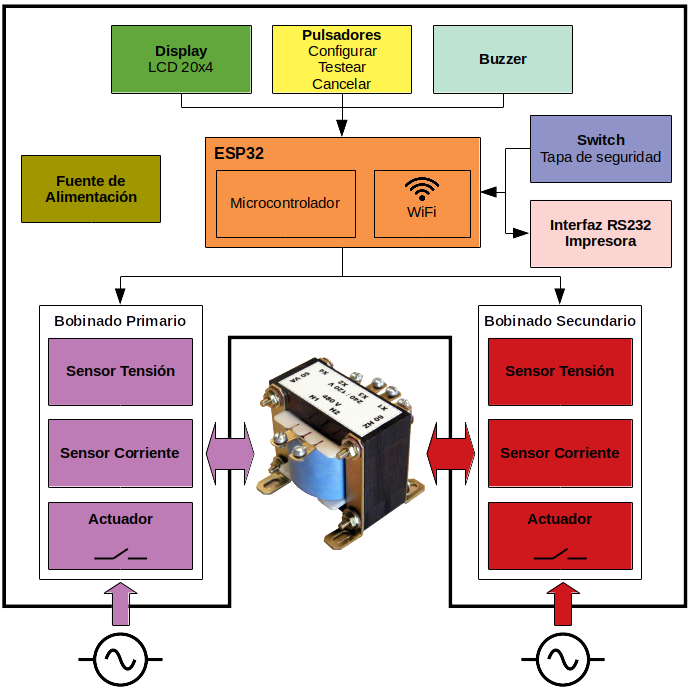
\includegraphics[width=.8\textwidth]{./Figuras/diagBloques.png}
\caption{Diagrama en bloques del sistema}
\label{fig:diagBloques}
\end{figure}

\section{Identificación y análisis de los interesados}
\label{sec:interesados}

\begin{consigna}{red} 
\begin{table}[ht]
%\caption{Identificación de los interesados}
%\label{tab:interesados}
\begin{tabularx}{\linewidth}{@{}|l|X|X|l|@{}}
\hline
\rowcolor[HTML]{C0C0C0} 
Rol           & Nombre y Apellido & Organización 	& Puesto 	\\ \hline
Cliente       & \clientename      &\empclientename	& Socio     \\ \hline
Responsable   & \authorname       & FIUBA        	& Alumno 	\\ \hline
Orientador    & \supname	      & \pertesupname 	& Director	Trabajo final \\ \hline
Usuario final & Operadores        &\empclientename	& Operador 	\\ \hline
\end{tabularx}
\end{table}
\end{consigna}



\section{1. Propósito del proyecto}
\label{sec:proposito}

El propósito de este proyecto es disminuir el riesgo de error humano y aumentar la fiabilidad de los datos obtenidos al evaluar los transformadores. Asimismo, se requiere aumentar la seguridad de los operadores expuestos a altas tensiones con la simplificación del procedimiento de caracterización y la incorporación de métodos de protección en el prototipo a diseñar.


\section{2. Alcance del proyecto}
\label{sec:alcance}

El presente proyecto tiene como alcance:
\begin{itemize}
\item Análisis, investigación y elección del hardware.
\item Investigar sobre un modelo de impresora a adquirir, cuyo protocolo esté disponible y permita llevar a cabo el proyecto.
\item Diseño e implementación del firmware del sistema en lenguaje C.
\item Desarrollo de un prototipo funcional sobre un PCB tipo universal.
\item Elaboración de un manual de usuario con la información mínima requerida para la operación del dispositivo y con las recomendaciones para evitar descargas de alta tensión. 
\end{itemize}

Queda excluido del alcance de este proyecto:
\begin{itemize}
\item El desarrollo de circuitos de medición de tensión y/o corriente alterna de precisión. Se acepta la precisión obtenida de módulos comerciales como el ZMPT101B.
\item El desarrollo de fuentes de tensión alterna para alimentar los transformadores en ensayo. El cliente deberá proporcionar al dispositivo los 230Vac estabilizados necesarios para alimentar el bobinado primario y la tensión alterna adecuada para alimentar el bobinado secundario.
\item El desarrollo de una interfaz web desde la cual interactuar por WiFi con el módulo.
\item El desarrollo del servidor web o API de colección de datos del en el servidor/PC del cliente. Esta será provista por el cliente.
\item El desarrollo de un prototipo de fabricación escalable que cumpla con todas las certificaciones necesarias.
\item El desarrollo de un PCB, más allá del prototipo en placa universal.
\item El diseño del gabinete para la instalación del sistema electrónico.
\item El diseño de circuitos de protección del operario contra descargas eléctricas de alta tensión. En este sentido, se asume que el operario que utilizará el dispositivo es idóneo en el tema. Asimismo, se asume que el cliente posee en sus instalaciones las medidas de seguridad pertinentes para el trabajo con altas tensiones, como disyuntores y puestas a tierras, acorde con la normativa vigente de Higiene y Seguridad en el Trabajo.
\end{itemize}

\section{3. Supuestos del proyecto}
\label{sec:supuestos}


Para el desarrollo del presente proyecto se supone que:

\begin{itemize}
\item La precisión necesaria para las mediciones de tensión y/o corrientes pueden ser obtenida con el uso de módulos comerciales como el ZMPT101B con modificaciones mínimas.
\item Los costos de los materiales serán cubiertos por el cliente.
\item Los materiales necesarios para el armado del prototipo pueden ser comprados en el país, aun con las restricciones de importación impuestas por el COVID-19.
\item El cliente proveerá los transformadores a medir.
\item El cliente proveerá la impresora a utilizar.
\item La impresora a utilizar posee interfaz RS-232.
\item El protocolo de la impresora a utilizar debe estar disponible para su implementación. No está contemplado dentro del proyecto hacer ingeniería inversa sobre la impresora a utilizar.
\item Si bien se incluyen algunas protecciones para el manejo de tensiones de 220 Vac, como se dijo anteriormente, se asume que el operario es idóneo y conoce los riesgos en la operación del dispositivo y que el cliente cumple las reglamentaciones de Higiene y Seguridad en el Trabajo.
\item El cliente es responsable de proporcionar, en caso de ser necesario y de una manera simple de entender e implementar, los requerimientos asociados al cumplimiento de su sistema de gestión de calidad para la fabricación de dispositivos médicos, basado en la norma ISO13485:2016 y cualquier otra normativa de cumplimiento necesario.
\end{itemize}



\section{4. Requerimientos}
\label{sec:requerimientos}


\begin{enumerate}
\item Requerimientos de hardware
	\begin{enumerate}
	\item El dispositivo debe ser diseñado en base al módulo ESP32.
	\item El dispositivo debe ser capaz de medir tensiones y corrientes alternas de manera aislada del transformador bajo ensayo.
	\item El dispositivo debe ser capaz de conmutar las tensiones primarias y secundarias.
	\item El dispositivo debe tener un display LCD alfanumérico 20x4 caracteres.
	\item El dispositivo debe tener una interfaz Wifi.
	\item El dispositivo debe tener una interfaz RS232 capaz de manejar impresoras.
	\item El dispositivo debe alimentarse desde la red eléctrica Argentina 220Vac/50hz, debiendo proveerse todas las alimentaciones a los diferentes módulos de hardware.
	\item El dispositivo debe poseer un \textit{switch} para indicar que la tapa de seguridad ha sido removida.
	\item El dispositivo debe poseer 3 pulsadores nombrados Configurar, Testear y Cancelar.
	\item El dispositivo debe poseer un \textit{buzzer}.
	\end{enumerate}
\item Requerimientos relativos a los valores a medir
	\begin{enumerate}
	\item Bobinado primario
		\begin{enumerate}
		\item Rango tensión: 100 – 240 Vac
		\item Rango corriente: 0 – 800 mAac
		\end{enumerate}
	\item Bobinado secundario
		\begin{enumerate}
		\item Rango tensión: 0 – 30 Vac
		\item Rango corriente: 0 – 1500 mAac
		\end{enumerate}
	\item Precisión en la medición de tensión: mejor al 1,5\% (puede variar en base a lo que se pueda conseguir en el mercado)
	\item Precisión en la medición de corriente: mejor al 4\% (puede variar en base a lo que se pueda conseguir en el mercado)
	\end{enumerate}
\item Requerimientos funcionales
	\begin{enumerate}
	\item El dispositivo debe permitir que se configuren los umbrales mínimos y máximos para los parámetros medidos. 
	\item Los valores a configurar deben ser adquiridos solo por WiFi, no se admite configuración local por teclado.
	\item El dispositivo debe generar una confirmación de aceptación o rechazo del transformador en ensayo basado en los umbrales mínimos y máximos preseteados.
	\item El dispositivo, luego de cada ensayo, independientemente del resultado, debe imprimir una etiqueta con la siguiente información:
		\begin{enumerate}
		\item Número de partida del transformador ensayado
		\item Condición de aceptado o rechazado
		\item Valores medidos de tensiones y corrientes
		\end{enumerate}
	\item El dispositivo debe seguir de forma automática la siguiente secuencia de testeo basico:
		\begin{itemize}
		\item Pulsar Testear
		\item Verificar si el dispositivo fue configurado, sino pedir parámetros de configuración
		\item Energizar el bobinado primario con 230Vac estabilizados  (provistos externamente por el cliente)
		\item Medir:
			\begin{itemize}
			\item Tensión en bobinado primario
			\item Corriente que circula por el bobinado primario
			\item Tensión en bobinado secundario
			\end{itemize}
		\item Desenergizar el bobinado primario
		\item Energizar el bobinado secundario con la tensión adecuada (provista externamente por el cliente)
		\item Medir:
			\begin{itemize}
			\item Tensión en bobinado primario
			\item Tensión en bobinado secundario
			\item Corriente que circula por el bobinado secundario
			\end{itemize}
		\item Desenergizar el bobinado secundario
		\item Comparar los valores medidos con los umbrales configurados previamente y determinar si el transformador es aceptado o rechazado
		\end{itemize}
	\end{enumerate}	
\item Requerimientos de comunicación (interfaz WiFi)
	\begin{enumerate}
	\item Solicitar parámetros de configuración: el dispositivo debe generar un comando GET de http a un servidor web (provisto por el cliente) para obtener los umbrales de aceptación y el número de partida del transformador a ensayar.
	\item El dispositivo debe ser capaz de procesar la respuesta del comando GET que estará en formato JSON.
	\item Enviar resultados del ensayo: el dispositivo debe generar un comando POST de http a un servidor (provisto por el cliente) con la información del transformador ensayado en formato JSON.
	\end{enumerate}
\item Requerimientos de interfaz de usuario
	\begin{enumerate}
	\item Sobre la funcionalidad de los pulsadores
		\begin{enumerate}
		\item Configurar: al pulsar este pulsador el dispositivo debe generar el comando GET para solicitar al servidor web los parámetros de configuración del dispositivo a través de WiFi.
		\item Testear: al pulsar este pulsador el dispositivo debe iniciar la secuencia de testeo.
		\item Cancelar: al pulsar este pulsador la secuencia de testeo en curso debe quedar abortada.
		\end{enumerate}
	\item Sobre la funcionalidad del display LCD
		\begin{enumerate}
		\item El dispositivo debe mostrar los umbrales presetedos y los valores de las mediciones actuales.
		\item Los valores de los umbrales configurados en el dispositivo deberán permanecer en el display  durante el ensayo.
		\item El dispositivo debe mostrar los valores medidos del transformador ensayado luego de cada medición.
		\item Luego de finalizado el ensayo se debe mostrar un mensaje que indique que la información del ensayo se ha enviado al servidor web y mantenerse el dispositivo bloqueado hasta que se haya recibido la respuesta del servidor.
		\end{enumerate}
	\item Sobre el \textit{buzzer}
		\begin{enumerate}
		\item El dispositivo debe emitir un solo sonido de 0,5 segundos de duración para confirmar la aceptación del transformador.
		\item El dispositivo debe emitir un sonido de repetición de 5 ciclos de 0,5 segundos de duración, con pausas de 0,5 segundos para confirmar el rechazo del transformador.
		\end{enumerate}		
	\end{enumerate}
\end{enumerate}



\section{Historias de usuarios (\textit{Product backlog})}

En esta sección se deben incluir las historias de usuarios y su ponderación (history points). Recordar que las historias de usuarios son descripciones cortas y simples de una característica contada desde la perspectiva de la persona que desea la nueva capacidad, generalmente un usuario o cliente del sistema. La ponderación es un número entero que representa el tamaño de la historia comparada con otras historias de similar tipo.

\label{sec:backlog}

\section{5. Entregables principales del proyecto}
\label{sec:entregables}


\begin{itemize}
\item Lista de componentes
\item Diagrama esquemático de la placa universal
\item Diagrama de cableado del dispositivo
\item Código fuente en C
\item Prototipo del equipo funcionando
\item Manual de uso
\item Informe final
\end{itemize}



\section{6. Desglose del trabajo en tareas}
\label{sec:wbs}


\begin{enumerate}
\item Análisis y definición de requerimientos (40 hs)
	\begin{enumerate}
	\item Definición del alcance y captura de requerimientos con el cliente (20 hs).
	\item Análisis de factibilidad: investigación sobre características de sensores de corriente alterna disponibles en el mercado (10 hs).
	\item Planificación del proyecto, escritura de documentos previos (10 hs).
	\end{enumerate}
\item Desarrollo de hardware (170 hs)
	\begin{enumerate}
	\item Cálculo, simulación y selección de los componentes de hardware (45 hs).
	\item Diseño del diagrama esquemático (25 hs).
	\item Gestión de compra de componentes con el cliente (15 hs).
	\item Armado de prototipo de hardware preliminar en protoboard (20 hs).
	\item Armado del circuito final en placa universal (40 hs).
	\item Ensamblado del prototipo (15 hs).
	\item Pruebas preliminares de hardware (10 hs).
	\end{enumerate}
\item Desarrollo de software (240 hs)
	\begin{enumerate}
	\item Preparación del entorno de trabajo, descarga e instalación de IDE y puesta punto del programador (5 hs).
	\item Diseño de la arquitectura de software (20 hs).
	\item Diseño de rutinas de medición (verdadero valor eficaz) (25 hs).
	\item Diseño de rutinas funcionales (40 hs).
	\item Diseño de rutinas de comunicación WiFi (40 hs).
	\item Desarrollo de la interfaz de usuario (40 hs).
	\item Investigación y desarrollo de bibliotecas para el manejo de la impresora (30 hs).
	\item Integración de las tareas en el RTOS (40 hs).
	\end{enumerate}
\item Verificación y validación del dispositivo (60 hs)
	\begin{enumerate}
	\item Desarrollo de pruebas unitarias (20 hs).
	\item Desarrollo de pruebas de integración de los componentes de hardware/software (20hs).
	\item Desarrollo de pruebas funcionales con diferentes transformadores (20 hs).
	\end{enumerate}
\item Cierre del proyecto (100 hs)
	\begin{enumerate}
	\item  Informes de avance del proyecto (10 hs).
	\item  Confección del manual de usuario (20 hs).
	\item  Memoria descriptiva final del proyecto (50 hs).
	\item  Elaboración de presentación final (20 hs).
	\end{enumerate}		
\end{enumerate}

Cantidad total de horas: (610 hs)

\newpage

\section{7. Diagrama de Activity On Node}
\label{sec:AoN}

\begin{figure}[htpb]
\centering 
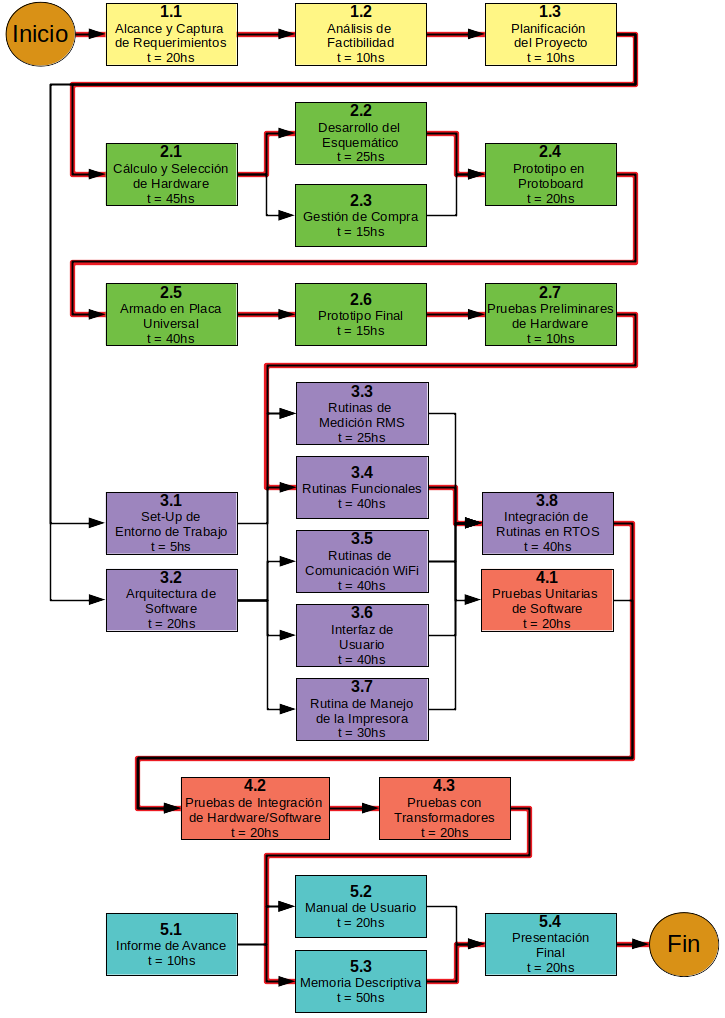
\includegraphics[width=.8\textwidth]{./Figuras/AoN.png}
\caption{Diagrama en \textit{Activity on Node}}
\label{fig:AoN}
\end{figure}



\begin{figure}[htpb]
\centering 
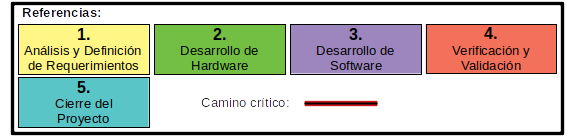
\includegraphics[width=.8\textwidth]{./Figuras/AoN_ref.png}
\caption{Referencias Diagrama en \textit{Activity on Node}}
\label{fig:AoN_ref}
\end{figure}


\newpage
\section{8. Diagrama de Gantt}
\label{sec:gantt}

\begin{figure}[htpb]
\centering 
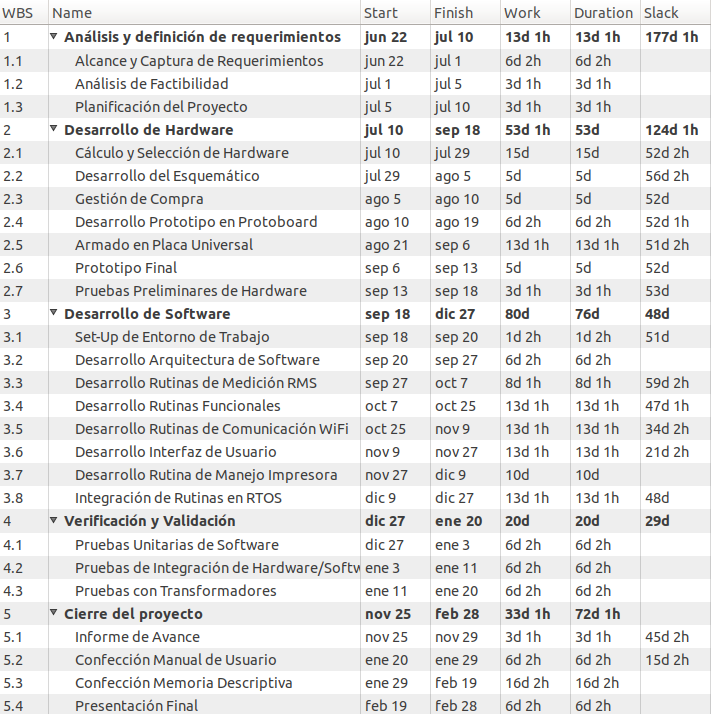
\includegraphics[width=.8\textwidth]{./Figuras/Gantt_1.png}
\caption{Diagrama de \textit{Gantt}}
\label{fig:Gantt_1}
\end{figure}

\begin{figure}[htpb]
\centering 
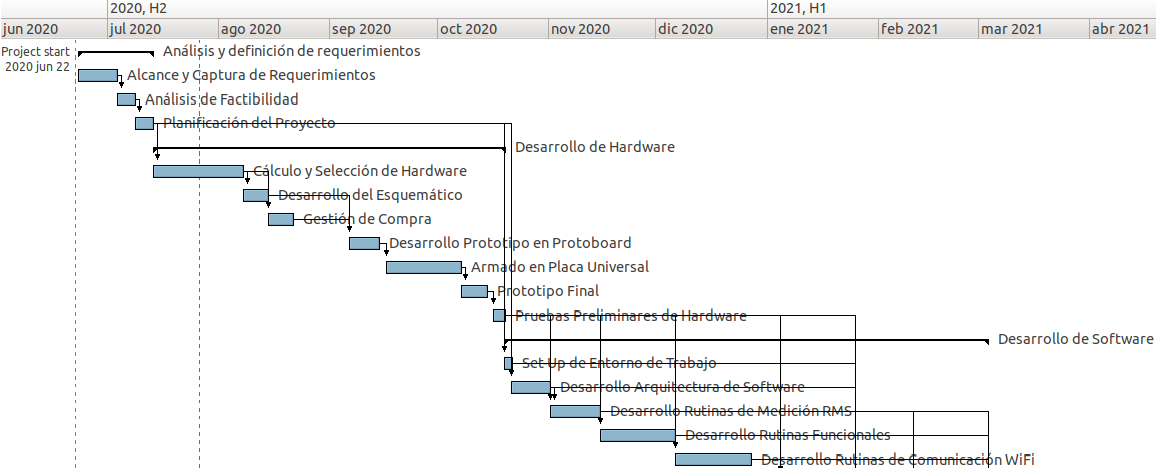
\includegraphics[width=.6\textwidth]{./Figuras/Gantt_2.png}
\caption{Diagrama de \textit{Gantt} Cont.}
\label{fig:Gantt_2}
\end{figure}

\newpage

\begin{figure}[htpb]
\centering 
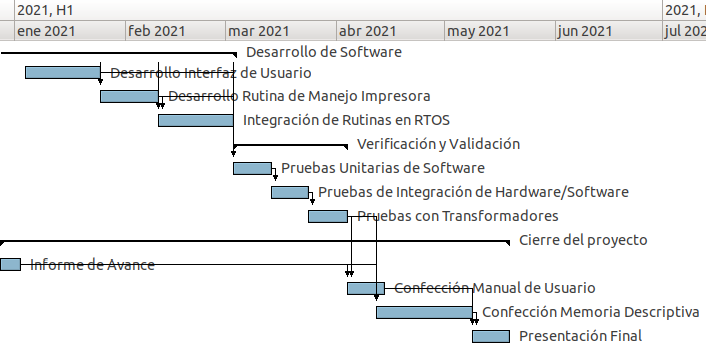
\includegraphics[width=.8\textwidth]{./Figuras/Gantt_3.png}
\caption{Diagrama de \textit{Gantt} Cont.}
\label{fig:Gantt_3}
\end{figure}

\section{9. Matriz de uso de recursos de materiales}
\label{sec:recursos}

\begin{table}[htpb]
\label{tab:recursos}
\centering
\begin{tabular}{|c|l|c|c|c|c|}
\hline
\cellcolor[HTML]{C0C0C0} & \multicolumn{1}{c|}{\cellcolor[HTML]{C0C0C0}{\color[HTML]{000000} }} & \multicolumn{4}{c|}{\cellcolor[HTML]{C0C0C0}Recursos requeridos (horas)}                                                                                                                                    \\ \cline{3-6} 
\multirow{-2}{*}{\cellcolor[HTML]{C0C0C0}\begin{tabular}[c]{@{}c@{}}Código\\ WBS\end{tabular}} & \multicolumn{1}{c|}{\multirow{-2}{*}{\cellcolor[HTML]{C0C0C0}{\color[HTML]{000000} \begin{tabular}[c]{@{}c@{}}Nombre\\ tarea\end{tabular}}}} & PC    & \begin{tabular}[c]{@{}c@{}}Equipamiento de \\ Laboratorio\end{tabular} & \begin{tabular}[c]{@{}c@{}}Prototipo\\ Protoboard\end{tabular} & \begin{tabular}[c]{@{}c@{}}Prototipo\\ Final\end{tabular} \\ \hline
1 & \begin{tabular}[c]{@{}l@{}}Análisis y definición\\ de Requerimientos\end{tabular} & 40  & & & \\ \hline
2 & Desarrollo de Hardware & 95  & 85 & 20 & 65 \\ \hline
3 & Desarrollo de Software & 240 & 100 & & 200 \\ \hline
4 & Verificación y Validación & 60  & 40 & & 60 \\ \hline
5 & Cierre del proyecto & 100 & 30 & & 30 \\ \hline
\end{tabular}
\end{table}

\newpage

\section{10. Presupuesto detallado del proyecto}
\label{sec:presupuesto}

\begin{table}[htpb]
\centering
\begin{tabularx}{\linewidth}{@{}|X|c|r|r|@{}}
\hline
\rowcolor[HTML]{C0C0C0} 
\multicolumn{4}{|c|}{\cellcolor[HTML]{C0C0C0}COSTOS DIRECTOS} \\ \hline
\rowcolor[HTML]{C0C0C0} 
Descripción &
  \multicolumn{1}{c|}{\cellcolor[HTML]{C0C0C0}Cantidad} &
  \multicolumn{1}{c|}{\cellcolor[HTML]{C0C0C0}Valor unitario} &
  \multicolumn{1}{c|}{\cellcolor[HTML]{C0C0C0}Valor total} \\ \hline
Placa de desarrollo ESP32 & \multicolumn{1}{c|}{1} & \multicolumn{1}{c|}{\$ 1620} & \multicolumn{1}{c|}{\$ 1620} \\ \hline
Sensor De Voltaje Alterna ZMPT101B 250V & \multicolumn{1}{c|}{2} & \multicolumn{1}{c|}{\$ 728} & \multicolumn{1}{c|}{\$ 1456} \\ \hline
Sensor De Corriente Alterna ZMCT103C & \multicolumn{1}{c|}{2} & \multicolumn{1}{c|}{\$ 1068} & \multicolumn{1}{c|}{\$ 2136} \\ \hline
Modulo Relé de 8 Canales & \multicolumn{1}{c|}{1} & \multicolumn{1}{c|}{\$ 1112} & \multicolumn{1}{c|}{\$ 1112} \\ \hline
Display LCD \textit{Backlight} Azul 20x4 & \multicolumn{1}{c|}{1} & \multicolumn{1}{c|}{\$ 1140} & \multicolumn{1}{c|}{\$ 1140} \\ \hline
Fuente \textit{Switching} AC-DC 5 V 700 mA & \multicolumn{1}{c|}{2} & \multicolumn{1}{c|}{\$ 370} & \multicolumn{1}{c|}{\$ 740} \\ \hline
Modulo Conector MAX3232 & \multicolumn{1}{c|}{1} & \multicolumn{1}{c|}{\$ 320} & \multicolumn{1}{c|}{\$ 320} \\ \hline
Componentes varios & \multicolumn{1}{c|}{1} & \multicolumn{1}{c|}{\$ 1648} & \multicolumn{1}{c|}{\$ 1648} \\ \hline
Placa Experimental Doble Faz 9x15cm & \multicolumn{1}{c|}{1} & \multicolumn{1}{c|}{\$ 569} & \multicolumn{1}{c|}{\$ 569} \\ \hline
Horas de ingeniería & \multicolumn{1}{c|}{600} & \multicolumn{1}{c|}{U\$S 8} & \multicolumn{1}{c|}{U\$S 4960(*)} \\ \hline
\multicolumn{3}{|c|}{SUBTOTAL} &
  \multicolumn{1}{c|}{\$ 361241} \\ \hline
\rowcolor[HTML]{C0C0C0} 
\multicolumn{4}{|c|}{\cellcolor[HTML]{C0C0C0}COSTOS INDIRECTOS} \\ \hline 
\rowcolor[HTML]{C0C0C0} 
\multicolumn{3}{|l|}{Descripción} & \\ \hline
\multicolumn{3}{|l|}{Estimados como el 40\% de los costos directos} & \multicolumn{1}{c|}{\$ 144496} \\ \hline
\multicolumn{3}{|c|}{SUBTOTAL} &
  \multicolumn{1}{c|}{\$ 144496} \\ \hline
\rowcolor[HTML]{C0C0C0}
\multicolumn{3}{|c|}{TOTAL} & \multicolumn{1}{c|}{\$ 505737}
   \\ \hline
\end{tabularx}%
\end{table}

(*) 1 U\$S = 73 \$, cotización al día Jueves 23 de Julio 2020

\newpage

\section{11. Matriz de asignación de responsabilidades}
\label{sec:responsabilidades}

\begin{table}[htpb]
\centering
\resizebox{\textwidth}{!}{%
\begin{tabular}{|c|c|c|c|}
\hline
\rowcolor[HTML]{C0C0C0} 
\cellcolor[HTML]{C0C0C0} & \multicolumn{1}{c|}{\cellcolor[HTML]{C0C0C0}{\color[HTML]{000000} }} & \multicolumn{2}{c|}{\cellcolor[HTML]{C0C0C0}Listar todos los nombres y roles del proyecto} \\ \cline{3-4} 
\rowcolor[HTML]{C0C0C0} 
\multirow{-2}{*}{\cellcolor[HTML]{C0C0C0}\begin{tabular}[c]{@{}c@{}}Código\\ WBS\end{tabular}} & \multicolumn{1}{c|}{\multirow{-2}{*}{\cellcolor[HTML]{C0C0C0}{\color[HTML]{000000} \begin{tabular}[c]{@{}c@{}}Nombre\\ tarea\end{tabular}}}} & \begin{tabular}[c]{@{}c@{}}Responsable\\ \authorname \end{tabular} & \multicolumn{1}{c|}{\cellcolor[HTML]{C0C0C0}{\color[HTML]{333333} \begin{tabular}[c]{@{}c@{}}Orientador/Cliente\\ \clientename \end{tabular}}} \\ \hline
1.1 & Alcance y Captura de Requerimientos     & P & A \\ \hline
1.2 & Análisis de Factibilidad                & P &   \\ \hline
1.3 & Planificación del Proyecto              & P & C \\ \hline
2.1 & Cálculo y Selección de Hardware         & P & C \\ \hline
2.2 & Desarrollo del Esquemático              & P &   \\ \hline
2.3 & Gestión de Compra                       & P & A \\ \hline
2.4 & Desarrollo Prototipo en Protoboard      & P &   \\ \hline
2.5 & Armado en Placa Universal               & P &   \\ \hline
2.6 & Prototipo Final                         & P & C \\ \hline
2.7 & Pruebas Preliminares de Hardware        & P & I \\ \hline
3.1 & Set-Up de Entorno de Trabajo            & P &   \\ \hline
3.2 & Desarrollo Arquitectura de Software     & P &   \\ \hline
3.3 & Desarrollo Rutinas de Medición RMS      & P &   \\ \hline
3.4 & Desarrollo Rutinas Funcionales          & P &   \\ \hline
3.5 & Desarrollo Rutinas de Comunicación WiFi & P &   \\ \hline
3.6 & Desarrollo Interfaz de Usuario          & P & C \\ \hline
3.7 & Desarrollo Rutina de Manejo Impresora   & P & C \\ \hline
3.8 & Integración de Rutinas en RTOS          & P & I \\ \hline
4.1 & Pruebas Unitarias de Software           & P &   \\ \hline
4.2 & Pruebas de Integración de Hardware/Software & P & \\ \hline
4.3 & Pruebas con Transformadores             & P & I \\ \hline
5.1 & Informe de Avance                       & P & A \\ \hline
5.2 & Confección Manual de Usuario            & P & A \\ \hline
5.3 & Confección Memoria Descriptiva          & P & A \\ \hline
\end{tabular}%
}
\end{table}


{\footnotesize
Referencias:
\begin{itemize}
	\item P = Responsabilidad Primaria
	\item S = Responsabilidad Secundaria
	\item A = Aprobación
	\item I = Informado
	\item C = Consultado
\end{itemize}
} %footnotesize


\section{12. Gestión de riesgos}
\label{sec:riesgos}

\begin{consigna}{red}
a) Identificación de los riesgos (al menos cinco) y estimación de sus consecuencias:
 
Riesgo 1: detallar el riesgo (riesgo es algo que si ocurre altera los planes previstos)
\begin{itemize}
\item Severidad (S): mientras más severo, más alto es el número (usar números del 1 al 10).\\
Justificar el motivo por el cual se asigna determinado número de severidad (S).
\item Probabilidad de ocurrencia (O): mientras más probable, más alto es el número (usar del 1 al 10).\\
Justificar el motivo por el cual se asigna determinado número de (O). 
\end{itemize}   

Riesgo 2:
\begin{itemize}
\item Severidad (S): 
\item Ocurrencia (O):
\end{itemize}

Riesgo 3:
\begin{itemize}
\item Severidad (S): 
\item Ocurrencia (O):
\end{itemize}


b) Tabla de gestión de riesgos:      (El RPN se calcula como RPN=SxO)

\begin{table}[htpb]
\centering
\begin{tabularx}{\linewidth}{@{}|X|c|c|c|c|c|c|@{}}
\hline
\rowcolor[HTML]{C0C0C0} 
Riesgo & S & O & RPN & S* & O* & RPN* \\ \hline
       &   &   &     &    &    &      \\ \hline
       &   &   &     &    &    &      \\ \hline
       &   &   &     &    &    &      \\ \hline
       &   &   &     &    &    &      \\ \hline
       &   &   &     &    &    &      \\ \hline
\end{tabularx}%
\end{table}

Criterio adoptado: 
Se tomarán medidas de mitigación en los riesgos cuyos números de RPN sean mayores a ....

Nota: los valores marcados con (*) en la tabla corresponden luego de haber aplicado la mitigación.

c) Plan de mitigación de los riesgos que originalmente excedían el RPN máximo establecido:
 
Riesgo 1: Plan de mitigación (si por el RPN fuera necesario elaborar un plan de mitigación).
  Nueva asignación de S y O, con su respectiva justificación:
  - Severidad (S): mientras más severo, más alto es el número (usar números del 1 al 10).
          Justificar el motivo por el cual se asigna determinado número de severidad (S).
  - Probabilidad de ocurrencia (O): mientras más probable, más alto es el número (usar del 1 al 10).
          Justificar el motivo por el cual se asigna determinado número de (O).

Riesgo 2: Plan de mitigación (si por el RPN fuera necesario elaborar un plan de mitigación).
 
Riesgo 3: Plan de mitigación (si por el RPN fuera necesario elaborar un plan de mitigación)

\end{consigna}


\section{13. Gestión de la calidad}
\label{sec:calidad}

\begin{consigna}{red}
Para cada uno de los requerimientos del proyecto indique:
\begin{itemize} 
\item Req \#1: Copiar acá el requerimiento.

Verificación y validación:

\begin{itemize}
\item Verificación para confirmar si se cumplió con lo requerido antes de mostrar el sistema al cliente:\\
Detallar 
\item Validación con el cliente para confirmar que está de acuerdo en que se cumplió con lo requerido:\\
Detallar  
\end{itemize}

\end{itemize}

Tener en cuenta que en este contexto se pueden mencionar simulaciones, cálculos, revisión de hojas de datos, consulta con expertos, etc.

\end{consigna}

\section{14. Comunicación del proyecto}
\label{sec:comunicaciones}

\begin{consigna}{red}
El plan de comunicación del proyecto es el siguiente:
\end{consigna}

% Please add the following required packages to your document preamble:
% \usepackage{graphicx}
% \usepackage[table,xcdraw]{xcolor}
% If you use beamer only pass "xcolor=table" option, i.e. \documentclass[xcolor=table]{beamer}
\begin{table}[htpb]
\centering
\resizebox{\textwidth}{!}{%
\begin{tabular}{|c|c|c|c|c|c|}
\hline
\rowcolor[HTML]{C0C0C0} 
\multicolumn{6}{|c|}{\cellcolor[HTML]{C0C0C0}PLAN DE COMUNICACIÓN DEL PROYECTO}           \\ \hline
\rowcolor[HTML]{C0C0C0} 
¿Qué comunicar? & Audiencia & Propósito & Frecuencia & Método de comunicac. & Responsable \\ \hline
                &           &           &            &                      &             \\ \hline
                &           &           &            &                      &             \\ \hline
                &           &           &            &                      &             \\ \hline
                &           &           &            &                      &             \\ \hline
                &           &           &            &                      &             \\ \hline
\end{tabular}%
}
\end{table}

\section{15. Gestión de Compras}
\label{sec:compras}

\begin{consigna}{red}
En caso de tener que comprar elementos o contratar servicios:
a) Explique con qué criterios elegiría a un proveedor.
b) Redacte el Statement of Work correspondiente.
\end{consigna}

\section{16. Seguimiento y control}
\label{sec:seguimiento}

\begin{consigna}{red}
Para cada tarea del proyecto establecer la frecuencia y los indicadores con los se seguirá su avance y quién será el responsable de hacer dicho seguimiento y a quién debe comunicarse la situación (en concordancia con el Plan de Comunicación del proyecto).

El indicador de avance tiene que ser algo medible, mejor incluso si se puede medir en \% de avance. Por ejemplo,se pueden indicar en esta columna cosas como ``cantidad de conexiones ruteadeas'' o ``cantidad de funciones implementadas'', pero no algo genérico y ambiguo como ``\%'', porque el lector no sabe porcentaje de qué cosa.

\end{consigna}

\begin{table}[!htpb]
\centering
\begin{tabularx}{\linewidth}{@{}|X|X|X|X|X|X|@{}}
\hline
\rowcolor[HTML]{C0C0C0} 
\multicolumn{6}{|c|}{\cellcolor[HTML]{C0C0C0}SEGUIMIENTO DE AVANCE}                                                                       \\ \hline
\rowcolor[HTML]{C0C0C0} 
Tarea del WBS & Indicador de avance & Frecuencia de reporte & Resp. de seguimiento & Persona a ser informada & Método de comunic. \\ \hline
 &  &  &  &  &  \\ \hline
 &  &  &  &  &  \\ \hline
 &  &  &  &  &  \\ \hline
 &  &  &  &  &  \\ \hline
 &  &  &  &  &  \\ \hline
\end{tabularx}%
%}
\end{table}

\section{17. Procesos de cierre}    
\label{sec:cierre}

\begin{consigna}{red}
Establecer las pautas de trabajo para realizar una reunión final de evaluación del proyecto, tal que contemple las siguientes actividades:

\begin{itemize}
\item Pautas de trabajo que se seguirán para analizar si se respetó el Plan de Proyecto original:
 - Indicar quién se ocupará de hacer esto y cuál será el procedimiento a aplicar. 
\item Identificación de las técnicas y procedimientos útiles e inútiles que se utilizaron, y los problemas que surgieron y cómo se solucionaron:
 - Indicar quién se ocupará de hacer esto y cuál será el procedimiento para dejar registro.
\item Indicar quién organizará el acto de agradecimiento a todos los interesados, y en especial al equipo de trabajo y colaboradores:
  - Indicar esto y quién financiará los gastos correspondientes.
\end{itemize}

\end{consigna}


\end{document}
